% !TEX root=template.tex

\typeout{NT FILE implementation.tex}

\prependtographicspath{{Chapters/Figures/}}

\glsresetall

%TODO: Maybe explain in way more detail the implementation? I can explain each agents implementation in more detail and add info on all the method? That feels excessive but it would increase page count I suspect

%O modelo de dados (?) todas as variáveis do programa desenvolvido

%Diagramas de classes com a implementação dos módulos e dos agentes

%Que interfaces existem entre os diferentes módulos, que dados são trocados nessas interfaces

%quais os métodos que são chamados quando uma sequência de execução de skill é feita

%quais os métodos quando um agente é lançado

%quais os behaviours utilizados para implementar os agentes

%quais as interações entre a tool que fizeste e o resto do ecossistema

%quais as libs que implementaste e como as fizeste (MQTT, HTTP, OPC UA)

\chapter{Implementation}
\label{cha:implementation}

Now that the architecture of the Module Engine and the accompanying \acrshort{MAS} has been laid out and well defined, it is time to implement it. First we will see exactly how each class works, their data models, methods and interfaces. Then we will explain what behaviours each agent makes use of, the methods used during setup and skill execution. Finally, we will see how the Module Engine interacts with the system and what Link Libraries were implemented.\\

\section{Class Implementations}
\label{sec:class_implementations}

For the implementation of the whole framework and accompanying \acrshort{MAS}, the Java programming language was selected. As mentioned in \ref{subsec:best_practices_and_common_architectures}, \acrshort{JADE} was built with the \acrshort{FIPA} specifications in mind and its Java version is well supported, so this framework was chosen to implement the \acrfull{MAS}.

The \acrshort{JADE} framework provides a lot of tools for agent development, communication and management. It provides a lot of classes and methods useful for agent setup, communication, \acrshort{DF} registration and more. Since this language was going to be used at length and is one of the best supported in the world, the Module Engine and the Link Libraries were also developed using it.\\

As mentioned in Chapter \ref{cha:architecture}, three main agent types were developed, \acrfullpl{RA}, \acrfullpl{TA} and \acrfullpl{PA}. Along with these, two more agents were created, \acrfull{PM} and \acrfull{DA}, with the purpose of launching and managing the other three agent types. All of these agents extend an interface "Agent" provided by \acrshort{JADE}.

This interface contains a lot of useful methods and variables, although not all of them are used in this \acrshort{MAS}. The methods used are the "setup" method, executed once when an agent is launched, and the "takeDown" method, executed when a agent is terminated. These methods must be overwritten to provide the agent with instructions on launch and termination.

Because the agents are launched through \acrshort{JADE}, the class constructor cannot have any initial arguments. To launch an agent with arguments, the method "getArguments" present in every agent can be used. It returns a generic object array the developed can then use to retrieve the arguments an agent is launched with.\\

\acrshort{JADE} also provides a lot of other classes that define agent behaviour. These classes must be defined inside the agents class to add new behaviours. Some of them must be used in order to make use of the different \acrshort{JADE} functionalities, like the Contract Net. Other simply exist to add a bit more flexibility during development.\\

The behaviour classes used in this project were:
\begin{itemize}
	\item The "OneShotBehaviour" class, that adds a single behaviour to the agents behaviour sequence. It is executed once, and then is excluded from the sequence;
	\item The "ContractNetInitiator" class, that allows an agent to start interacting with other agents as the Initiator in the Contract Net protocol;
	\item The "ContractNetResponder" class, that allows an agent to respond to messages as one of the Participants in the Contract Net protocol;
	\item The "AchieveREInitiator" class, that allows an agent to start interacting with anoter agent as the Initiator in the Requests protocol;
	\item And the "AchieveREResponder" class, that allows an agent to respond to messages as a Participant in the Requests protocol.
\end{itemize}

\subsection{Product Agent Class}
\label{subsec:product_agent}

The \acrlong{PA} class extends the "Agent" abstract class and overrides the "setup" and "takeDown" methods. It makes use of the "addBehaviour" and "getArguments" methods, as well as the "OneShotBehaviour", "ContractNetInitiator" and "AchieveREInitiator" classes. It also uses the auxiliary "Constants" and "DFInteraction" classes that are explained in \ref{subsec:constants} and \ref{subsec:directory_facilitator}, respectively.

It has an ArrayList of Strings called "executionPlan" to store the whole skill sequence, an int called "step" to store the current step in that sequence and a String "location" that stores the agents current location on the physical system.\\

The "executeNextSkill" class extends the "OneShotBehaviour" class, the "contractNetInitiator" class extends the "ContractNetInitiator" class and the "requestTransportMove" and "requestStationSkill" classes extend the "AchieveREInitator" class. These classes and methods are all represented in Figure~\ref{fig:pa_class_diagram}, along with the variables they use.\\

\begin{figure}[h!]
	\centering
	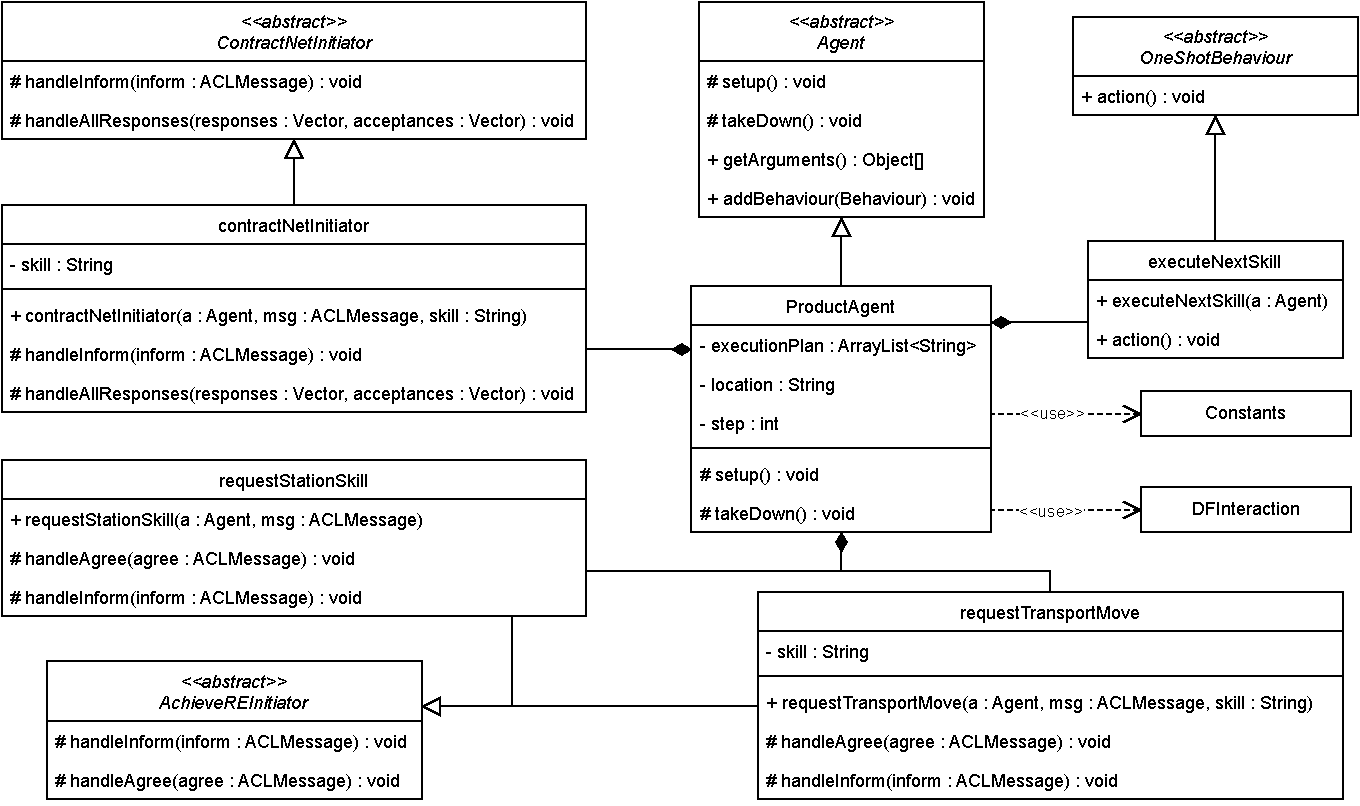
\includegraphics[scale=0.65]{PA_Class_Diagram}
	\caption{\acrlong{PA} class diagram.}
	\label{fig:pa_class_diagram}
\end{figure}

\subsection{Resource Agent Class}
\label{subsec:resource_agent}

The \acrlong{RA} class also extends the "Agent" abstract class and overrides the "setup" and "takeDown" methods as well. It makes use of the "addBehaviour" and "getArguments" methods for the same purposes, as well as the "ContractNetResponder" and "AchieveREResponder" classes.

Like the \acrshort{PA}, it also makes use of the auxiliary "Constants" and "DFInteraction" classes. It has two objects of type File called "xmlConfigFile" and "xmlMarketplaceFile that store the corresponding files. The String "libType" contains the type of Link Library this agent is using and the String "location" contains the position of this agent in the physical system.

Finally, the object "moduleEngine" of type ModuleEngine holds the Module Engine instance this agent is using, and the ArrayList of Strings "associatedSkills" holds the list of all skills this agent is able to perform.

The "requestResponder" class extends the "AchieveREResponder" class and the "contractNetResponder" class extends the "ContractNetResponder" class. Figure~\ref{fig:ra_class_diagram} shows a class diagram of the agent. In this Figure, the Module Engine and all subsequent classes are omitted, as they will be explained in \ref{subsec:module_engine} in more detail.\\

\begin{figure}[H]
	\centering
	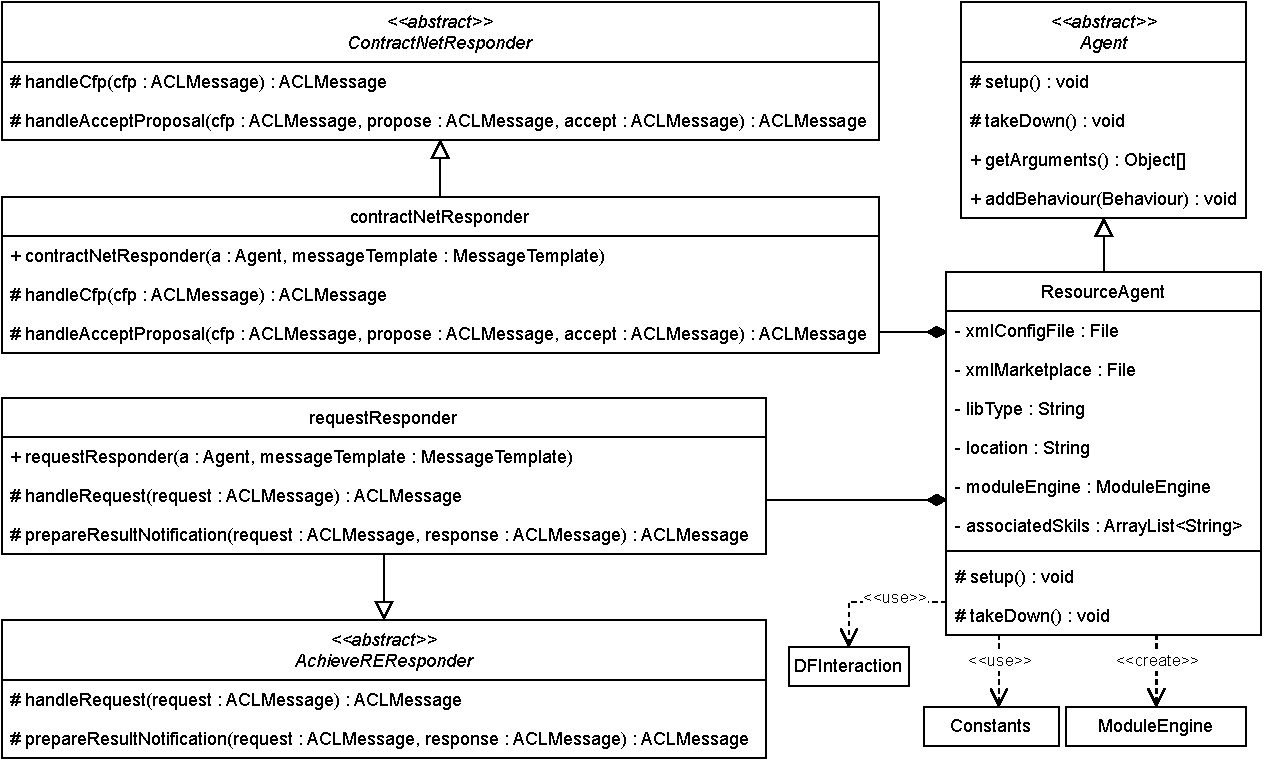
\includegraphics[scale=0.71]{RA_Class_Diagram}
	\caption{\acrlong{RA} class diagram.}
	\label{fig:ra_class_diagram}
\end{figure}

\subsection{Transport Agent Class}
\label{subsec:transport_agent}

The \acrlong{TA} class is very similar to the \acrlong{RA}. The only differences are in variables it uses and the classes it implements. It holds the same variables except for the "location", since the \acrlong{TA} does not have a location in the physical system. It contains both "setup" and "takeDown" methods. This class also makes use of the "Constants" and "DFInteraction" classes.\\

It implements a single "requestResponder" class which extends the "AchieveREResponder" class provided by \acrshort{JADE}.
Figure~\ref{fig:ta_class_diagram} has a representation of its implementation. Once again the classes related to the Module Engine have been omitted.\\

\begin{figure}[h!]
	\centering
	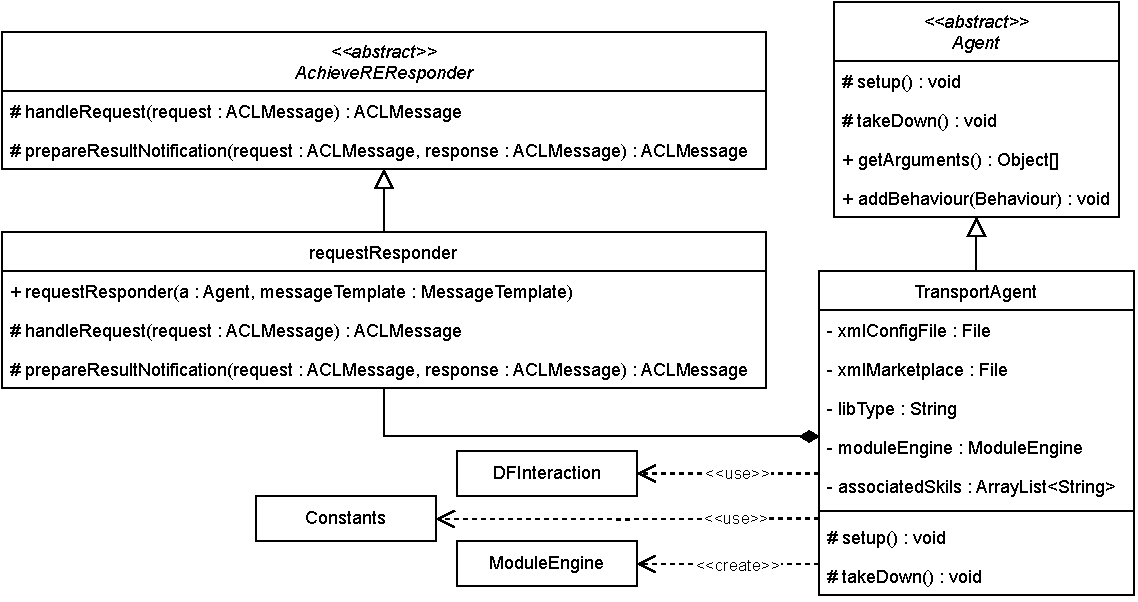
\includegraphics[scale=0.75]{TA_Class_Diagram}
	\caption{\acrlong{TA} class diagram.}
	\label{fig:ta_class_diagram}
\end{figure}

\subsection{Deployment Agent Class}
\label{subsec:deployment_agent}

The \acrlong{DA} class was designed to allow a human user to deploy and terminate agents during the execution of the \acrshort{MAS}. In its constructor the functionalities of the \acrshort{GUI} are defined and some initial values are set. This class extends the "Agent" class, and only makes use of the "setup" method. All other functionalities are called on button presses, through events.

The "selectedAgent" specifies which type of agent (\acrshort{RA} or \acrshort{TA}) is to be launched. This can be changed through a radio button on the interface.

The "xmlMarketplace" is loaded during "setup" with the method "getMarketplaceLibraries", using the file pointed to by the "marketplaceXMLPath" String. It holds the path of the \acrshort{XML} file that contains the available Link Libraries.

The "agentContainer" field holds a reference to the container where the agents deployed will be hosted. Finally, the "xmlConfigPath" is a user loaded value that is used to pass the Link Library configurations file.\\

In Figure~\ref{fig:da_class_diagram}, we can see some of the classes the agent uses to draw the \acrshort{GUI}. These classes are part of the "javax.swing" package, useful to draw graphic interfaces. as the "ContainerController" used to create a container where other agents are deployed. This is a \acrshort{JADE} class. We can also see the auxiliary "Constants" class, that stores constants useful for the correct operations of the \acrshort{MAS}. This class is defined in \ref{subsec:constants}.\\

\begin{figure}[h!]
	\centering
	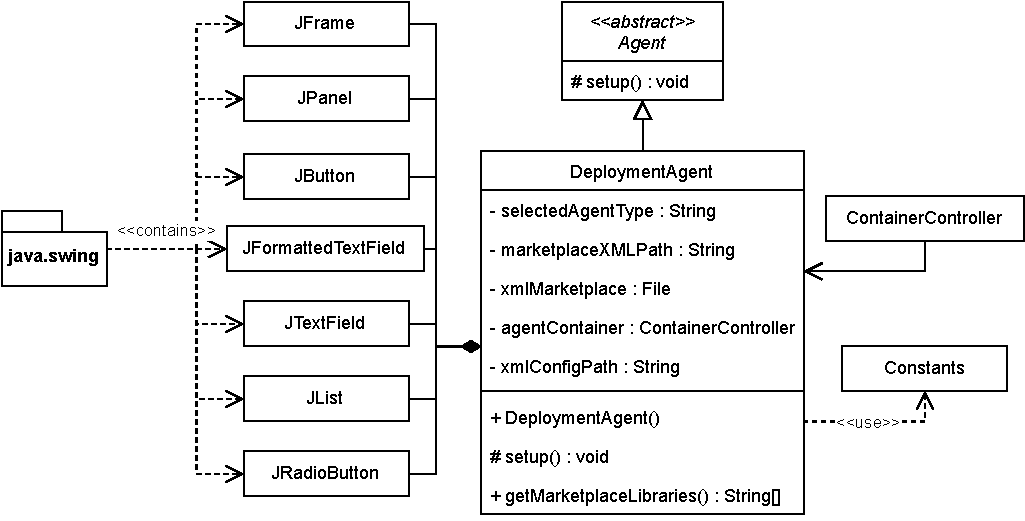
\includegraphics[scale=0.9]{DA_Class_Diagram}
	\caption{\acrlong{DA} class diagram.}
	\label{fig:da_class_diagram}
\end{figure}

\subsection{Product Manager Class}
\label{subsec:product_manager_agent}

This class also presents a \acrshort{GUI} to allow a human operator to launch \acrlongpl{PA}, although it cannot terminate them. It operates similarly to the \acrshort{DA}. This class also extends the "Agent" class, and also only makes use of the "setup" method.\\

In Figure~\ref{fig:pm_class_diagram}, the classes that it uses to draw the \acrshort{GUI} are shown, once again the "ContainerController" class to instantiate a container where \acrlongpl{PA} are launched. The "DefaultTableModel" class helps with the definition of the \acrshort{GUI}, and is a class in the "javax.swing" package.\\

\begin{figure}[h!]
	\centering
	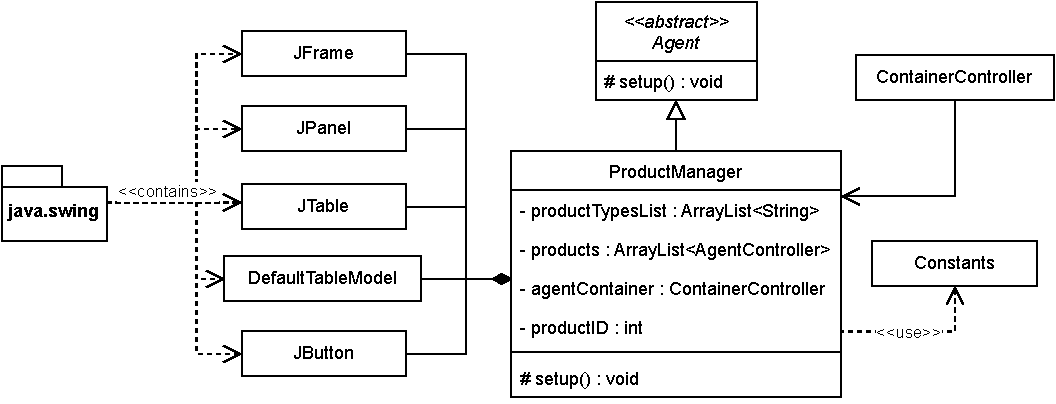
\includegraphics[scale=0.8]{PM_Class_Diagram}
	\caption{\acrlong{PM} class diagram.}
	\label{fig:pm_class_diagram}
\end{figure}


\subsection{Constants Class}
\label{subsec:constants}

To help define all of the constants needed for the \acrshort{MAS}, an auxiliary class of constants was created. This "Constants" class also contains a few methods to help with information retrieval. It is mostly composed of String fields. Other classes can reference it to check production sequences, locations, skills, etc. All of this information is visible in Figure~\ref{fig:const_class_diagram}.

\begin{figure}[h!]
	\centering
	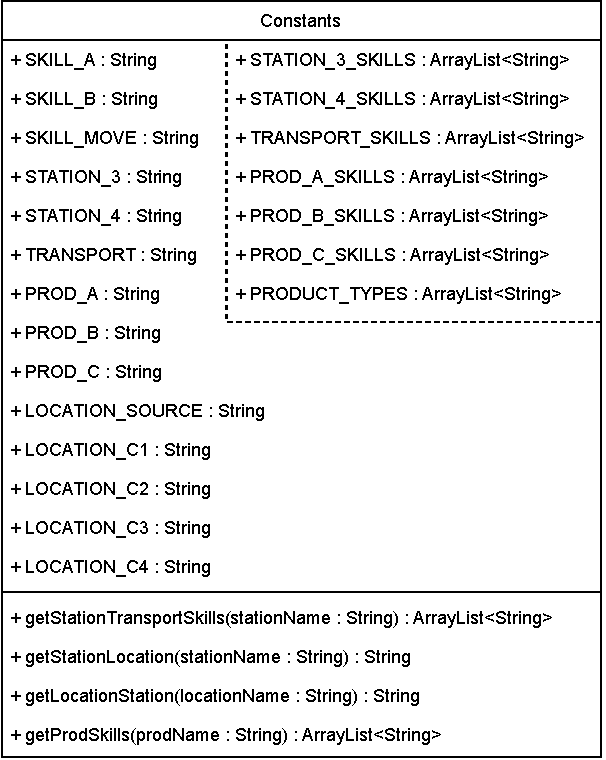
\includegraphics[scale=0.70]{Const_Class_Diagram}
	\caption{Constants class diagram}
	\label{fig:const_class_diagram}
\end{figure}

\subsection{Directory Facilitator Class}
\label{subsec:directory_facilitator}

The \acrlong{DF} class is another auxiliary class. It provides methods that can register, remove or search information on the \acrshort{DF}. Figure~\ref{fig:df_class_diagram} shows its diagram. The method "RegisterInDF" has two version, one allows for the registry of an agent with a single skill, the other for an agent with multiple skills. The "DFService" class is implemented by \acrshort{JADE} and it is what allows for the interactions with the \acrshort{DF}.\\

\begin{figure}[h!]
	\centering
	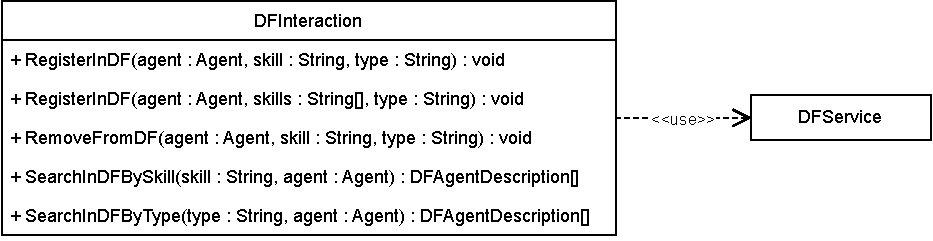
\includegraphics[scale=1]{DF_Class_Diagram}
	\caption{\acrlong{DF} class diagram}
	\label{fig:df_class_diagram}
\end{figure}

\subsection{Module Engine Class}
\label{subsec:module_engine}

With the whole \acrshort{MAS} already defined, we can now take a look at the hardware interface. The Module Engine class is the main framework that was developed for this. It contains a generic object "linkLibrary" that hold the currently loaded Link Library. It also has a "classesToLoad" Hashmap, which holds all the available Link Libraries, for quick access. This Hashmap is loaded with the method "parseMarketplaceXML".

The method "parseMarketplaceXML" does exactly that, it parses the file and loads the Link Libraries in the "classesToLoad" hashmap. This marketplace file is in the \acrshort{XML} format, and holds both the name of the Link Library and the class file that implements it. These are loaded by using the Reflections feature of the Java language. It allows for a program to inspect itself, and more importantly, to load classes and call their methods during runtime. This is what allows the Module Engine to load any kind of library at any point, while the \acrshort{MAS} is running.

The method "createObject" the String "libType", from the agent, that contains the type of Library to load. This library is then fetched from the "classedToLoad" Hashmap and attributed to a generic object of type "Class", or "Class<?>". This is then loaded using Reflections by creating a new object of that class and passing along the \acrshort{XML} configurations file, also received from the agent.

To execute a skill the method "executeSkill" is called, which will in turn get the method "ExecuteSkill" from the "linkLibrary" object and place it in a "Method" type object. This method is then invoked to execute the skill, which is passed as an argument, and its return message is returned as a String.

Finally, the method "shutdown" is used to disconnect the hardware from the Link Library, and is usually called when the agent, and consequently the Module Engine, is terminated. Figure~\ref{fig:module_engine_class_diagram} shows how this class is implemented, along with an example \acrshort{HTTP} Link Library.\\

\begin{figure}[h!]
	\centering
	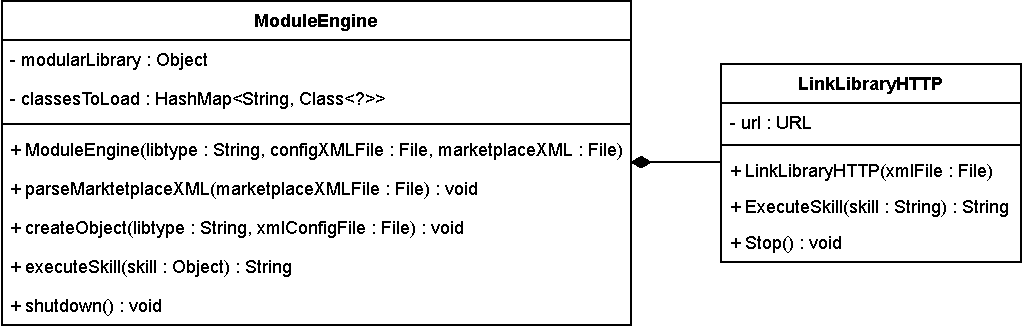
\includegraphics[scale=0.85]{ME_Class_Diagram}
	\caption{Module Engine class diagram}
	\label{fig:module_engine_class_diagram}
\end{figure}

\subsection{Link Library Classes}
\label{subsec:link_library_class}

To showcase the functionalities of the Module Engine, three different Link Libraries were developed. An abstract class "LinkLibrary" was extended to implement the "LinkLibraryHTTP", "LinkLibraryMQTT" and "LinkLibraryOPCUA" classes.

The "LinkLibraryHTTP" was implemented with the classes and methods provided in the "java.net" package. The "LinkLibraryMQTT" used the "org.eclipse.paho.client.mqttv3" package to implement its protocol and the "LinkLibraryOPCUA" used the "org.eclipse.milo.opcua" package.

All Link Libraries must extend the "LinkLibrary" class, because this is the basis of a Link Library and it defines the methods on which the Module Engine depends on for correct execution.

Figure~\ref{fig:link_library_class_diagram} has a representation of these classes and the respective packages they use to implement their communication protocols.\\

\begin{figure}[h!]
	\centering
	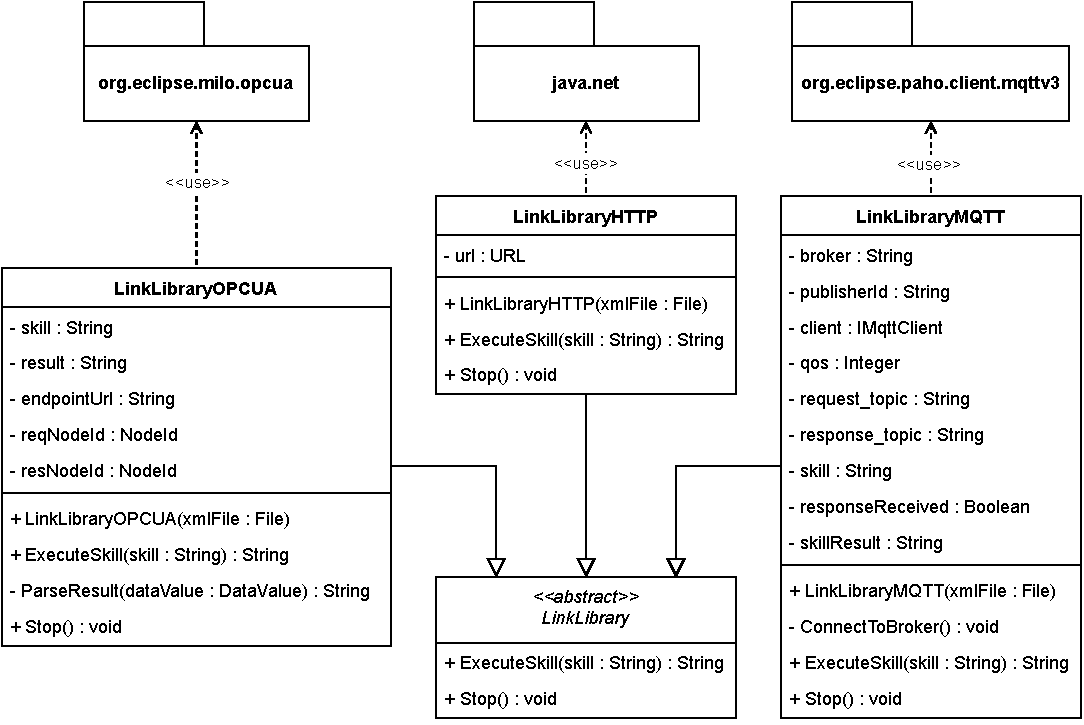
\includegraphics[scale=0.8]{LL_Class_Diagram}
	\caption{Link Library class diagrams}
	\label{fig:link_library_class_diagram}
\end{figure}

\section{Interfaces}
\label{sec:interfaces}

\subsection{Human to Agent}
\label{subsec:human_to_agent_interface}

As mentioned before, there are two agents with \acrlongpl{GUI}. The \acrlong{DA} and \acrlong{PM} both present a human user with an interface for agent deployment.

On the left side the \acrshort{DA} interface has a button to open a configuration file and a text box where the path to the currently chosen file appears. Then it has a text field where the agent name is written and two radio buttons where the agent type can be selected, \acrlong{RA} and \acrlong{TA}. Finally there is a list of all available libraries that are fetched from the marketplace file and a button that starts the agent. On the right side there is a list with the currently running \acrshortpl{RA} and \acrshortpl{TA}. These agents can be selected by clicking on them and stopped by pressing the stop agent button below the list. Figure~\ref{fig:da_gui} shows this interface.\\

\begin{figure}[h!]
	\centering
	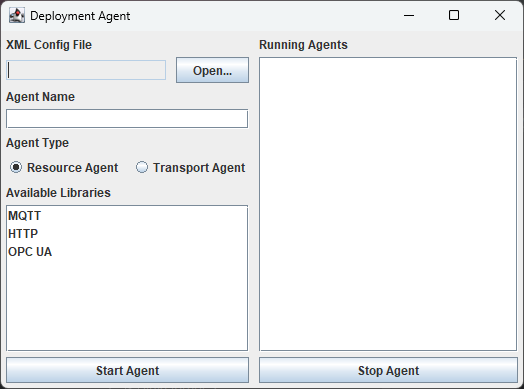
\includegraphics[scale=0.75]{DA_GUI}
	\caption{\acrlong{DA} \acrlong{GUI}.}
	\label{fig:da_gui}
\end{figure}

The \acrshort{PM} is more simple. It has buttons equivalent to the number of product agents specified in the "Constants" class and a list with the already launched agents. These agents have an ID represented by an integer, their product type and the skill sequence they need executed to complete the production process. We can see this interface in Figure~\ref{fig:pm_gui}.

\begin{figure}[h!]
	\centering
	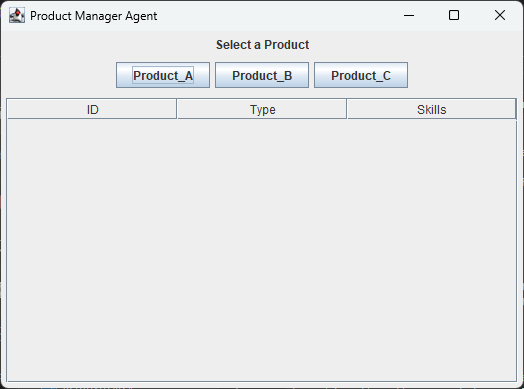
\includegraphics[scale=0.75]{PM_GUI}
	\caption{\acrlong{PM} \acrlong{GUI}.}
	\label{fig:pm_gui}
\end{figure}

\subsection{Agent to Agent}
\label{subsec:agent_to_agent_interface}

Agent to agent communication is done through ACLMessages. These have been defined by \acrshort{FIPA} \cite{FIPA_ACLMessage}. These messages have many parameters that help define communications. Table~\ref{tb:aclmessage_parameters} shows the parameters used by the agents of the \acrshort{MAS}, along with their utility.

\begin{table}[h!]
	\centering
	\caption{ACLMessage parameters}
	\begin{tabular}{|c|c|}
		\hline
		Parameter    & Utility                   \\ \hline
		performative & Type of communicative act \\ \hline
		sender       & Sender of the message     \\ \hline
		receiver     & Receiver of the message   \\ \hline
		content      & Content of the message    \\ \hline
	\end{tabular}
	\label{tb:aclmessage_parameters}
\end{table}

\subsection{Agent to Hardware}
\label{subsec:agent_to_hardware_interface}

To interface with the hardware, an agent must call the "executeSkill" method of the Module Engine. In its parameters it should send the skill as a String. The Module Engine will then call the "ExecuteSkill" of the Link Library loaded by it. All Link Libraries must contain the method "ExecuteSkill", otherwise calling it would be impossible. This method is implemented by the abstract class "LinkLibrary", as described in \ref{subsec:module_engine}.

The Link Library will now forward the skill through the protocol it is implementing, in whatever format it was designed for. A developer could reformat this message to whatever type they want, but the Link Library must always return a result of type String. As long as these rules are obeyed, Link Libraries can be used in the way most suitable to the system they are in. The result is passed to the Module Engine as a String, which is then passed to the agent.\\

Three Link Libraries were implemented, seen in \ref{subsec:link_library_class}. The \acrshort{HTTP} library works by creating an \acrshort{HTTP} connection, every time a skill is to be executed, using the address provided in the configurations. It sends the skill as a payload in a POST request. It then waits for an OK message with code 200 as per the \acrshort{HTTP} protocol. This response must include the result of the operation that is converted into a String and passed upward to the Module Engine. This library does not need to disconnect from the \acrshort{HTTP} server, since this protocol does not depend on a persistent connection.\\

The implemented \acrshort{MQTT} library needs more parameters to work. It requires an \acrshort{MQTT} broker address, a \acrfull{Quality of Service} value, a request topic and a response topic. These topics are differentiated to allow for a simpler implementation of the library. When the library is loaded, it immediately establishes a connection to the broker and immediately subscribes to the response topic. This means that every time a response arrives, the callback function is called. This function simply stores the message as a String. Whenever the "ExecuteSkill" method is run, the library will publish the skill in the request topic. It then waits until the response topic gets a message. Upon receiving it, it will return it to the Module Engine. When this library needs to disconnect, it just disconnects from the broker.\\

%TODO: Explain OPCUA in State of the Art?

The \acrshort{OPCUA} library is a bit more complex than the other two. It also needs a server address, or endpoint, and a namespace. This namespace identifies which container the node representing the hardware is. In this node, two variable nodes are found, one for incoming requests and one for outgoing responses. To summarize, the library needs and endpoint address, a namespace, the identifier of the request node and the identifier response node.

When the Link Library is loaded, it immediately connects to the \acrshort{OPCUA} server and creates two node objects with the namespace and one with the request and one with the response identifier. 




 \acrshort{OPCUA} works by creating a server. In this server there are many different folders. This Link Library assumes there is a folder 

%TODO: Explain Link Library implementations as interfaces to the hardware



\section{Multi-agent System Operations}
\label{sec:mas_operations}

With the whole system now defined, we can proceed to 